\chapter{Context and Background Information}
% This chapter should cover background information, related work, research
% done, and tools or software selected for use in the project.
% – Provide necessary context and background information to describe
% how your project relates to what is already known or available.
% – A description of the research carried out to learn out about the nature
% of the problem(s) being investigated and potential solutions. The form
% of the research will vary widely depending on the kind of project. For
% example, it might involve searching through research publications and
% online resources, or might involve an exploration of design
% possibilities for a user interface or program structure.
% – The sources of information you are drawing on (papers, books,
% websites, etc.) should all be cited or referenced clearly. In addition,
% state how each source relates to your work and avoid the temptation
% to pad out the chapter by including sources that you didn’t make use
% of during the project.
% – If relevant, a survey of similar solutions, programs or applications to
% yours, and how yours is differentiated.
% – Introduce the software, programming languages, library code,
% frameworks and other tools that you are using. Discuss choices and
% make clear which you made use of and why.
% You should not include well known things (e.g., HTML or Java) or try to give
% tutorials on how to use a tool or code library (use references to books and
% websites for that information). Everything you include should be directly
% relevant to your work and the relationship made clear. This chapter is likely
% to be fairly substantial, perhaps 8-10 pages.

% You should provide enough background to the reader for them to understand what the project is all about. For example:
% • What problem are you solving?
% • Why are you solving it?
% • How does this relate to other work in this area?
% • What work does it build on?
% • What is the scope of your work?
% • What is included in the scope and what is outside the scope?

\section{Background Information}
\subsection{OpenVINO}
The Intel Open Visual Inference and Neural Network Optimization (OpenVINO) toolkit is an open-source software stack designed to facilitate the rapid optimisation and deployment of machine learning models on Intel AIPC hardware\cite{intel_openvino_genai_workflow_2026}. Although the original release in May 2018 focused on computer vision tasks, it has received yearly updates following industry movement towards LLMs and generative AI\cite{intel_openvino_launch_2018}. One large benefit of this toolkit is the `optimum-cli` tool, enabling the download, quantisation, and conversion to OpenVINO intermediate representation (OpenVINO IR)\cite{intel_openvino_gaudi_aipc_2024}. The tool converts any huggingface model to OpenVINO IR format. If quantisation is required, it uses the Neural Network Compression Framework to reduce the mathematical precision of the model's weights, reducing the storage size and inference time with a negligible trade-off of inference accuracy\cite{hybrid_llm_openvino_2024}. It then exports the model into a .xml file mapping the network configuration and a .bin file containing the model's weights to satisfy the OpenVINO IR format. The OpenVINO inference engine executes the OpenVINO IR model using an optimised C++ engine directly interacting with low level hardware instruction sets on Intel's AIPC system-on-a-chip (SOC) architecture\cite{intel_openvino_inference_engine_2023}.

\subsection{Intel AI PC}
The Intel AIPC series was launched in December 2023 transitioning away from the old architectures of separately dedicated CPU, GPU and RAM components and moving towards a SOC design\cite{intel_meteor_lake_2023} where the previous components and new Neural Processing Unit (NPU) all live on the same combined chip stack by the release of the Lunar Lake series in late 2024. The NPU was a new computational unit specialised for low power matrix computation, designed as a device for low power inference of small ML models\cite{intel_lunar_lake_2024}. When paired with the native OpenVINO inference engine, the Intel AIPC is a strong candidate to provide a proof-of-concept for locally hosted ML pipelines\cite{fei2024_nitro_openvino}.

\subsection{Ambient Voice Technology}
Ambient Voice Technology (AVT) is an umbrella term for the field of passive automated note taking during conversations. The standard pipeline is as follows:

\begin{figure}
    \centering
    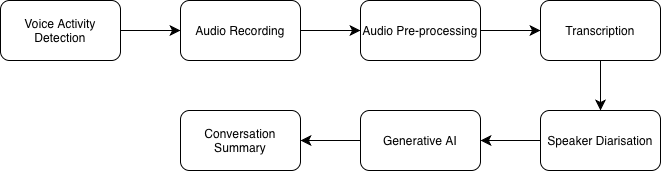
\includegraphics[width=1\linewidth]{AVT_diagram.drawio.png}
    \caption{A typical AVT workflow}
    \label{fig:AVT_diagram}
\end{figure}

This pipeline takes an audio stream as input, providing a summary as output \cite{lakhani_ai_scribes_2025}. Within the medical section this pipeline has been implemented with specialised speech-to-text and summarisation models to produce standardised medical documentation from a medical conversation \cite{tortus_product_2026}

\subsection{RAG}
Retrieval Augmented Generation (RAG) is a technique that enhances generative model outputs by first retrieving contextually relevant information from an external knowledge base and conditioning the model's generation on that retrieved context\cite{lewis_rag_2020}. This addresses a fundamental limitation of parametric LLMs. Since knowledge is fixed at training time, reliable access to domain specific or recently updated information is impossible without model retraining. The retrieval stage converts both the query and the knowledge base documents into dense vector representations (embeddings) using a semantic encoder. These embeddings capture the contextual meaning of text, enabling semantically similar passages to be located without exact keyword overlap. An approximate nearest neighbor (ANN) algorithm then searches the embedding index to surface the most contextually relevant document chunks\cite{malkov_hnsw_2020}. The retrieved chunks are passed to the LLM as additional context, enabling grounded responses anchored in verified source documents and significantly reducing the hallucination of domain-specific facts\cite{gao2023retrieval}. 

\subsection{NHS Appraisals}
Medical appraisals are an annual meetings with a supervisor aimed at retrospectively assessing challenges and lessons learnt from a personal development plan\cite{nhs_england_what_is_appraisal}. During this process, doctors must review their practice, evaluate patient and colleague feedback, and establish continuous personal development plans \cite{gmc_appraisal_guidance}. A method of reviewing their practice is through ad-hoc notes on specific consultations. An AVT solution can alleviate some of the pressure of gathering supporting information from consultations by storing reflection notes until an appraisal is required. This integration was requested by Dr. Atia Rafiq to aid her trainee GP's through this process

\subsection{Project Ambience (LLMedic)}
The prequel to this project, developed over the summer 2025 at UCL, hosted the Med42-70B model used for medical summarisation on Intel's GAUDI compute servers designed for AI acceleration on Intel hardware\cite{intel_gaudi3_2025}. This project acted as a proof-of-concept for running large AI fine-tuned medical models on Intel hardware using a web application for a client-server distribution model. The main shortfall was the hosting architecture as this server has open access to UCL students on a root level account, resulting in a solution too insecure to handle sensitive data. To remedy this, the project requires moving this model to an offline, on-device solution \cite{intel_openvino_gaudi_aipc_2024} while extending the summarisation pipeline with an AVT approach, appraisal entry system and RAG for medical advice. 

\section{Evaluation of Similar Solutions}
Evaluating the capabilities and shortfalls is essential to building a unique application that can capture the pain points of the current applications available to enable this proof of concept project to target a gap in the market. Furthermore, by analysing the current solutions, this project can position itself to develop on the successes that other applications have achieved in this growing field. 

\subsection{TORTUS AI}
TORTUS AI is an ambient medical scribe developed for the NHS as part of Great Ormond Street Hospital's (GOSH) drive for digital innovation involving a pipeline of machine learning models achieving an AVT and AI-scribe solution with complete integration into the GOSH EMIS EPR system\cite{tortus_product_2026}. This solution creates a "clinician in the loop" to systematically categorise LLM errors into risk levels targeting hallucinations and omissions from summaries during the training of their summarisation model on 13000 clinician annotated statements\cite{tortus_creola_2026}. Rollouts of this solution have shown a 23.5\% increase in face to face interaction between patients and doctors during consultations with an 8.2\% decrease in consultation length\cite{gosh_implementing_ai_2025}. In high pressure environments such as A\&E, the deployment of this solution enabled doctors to treat 13.4\% more patients per shift\cite{nia_tortus_2025}. Overall this is the leading solution for AVT and AI-scribe technologies in the NHS.

Considering the features of this project's solution, TORTUS AI does not support functionality for citing medical guidelines, or an appraisal entry solution. Furthermore, the key differentiating factor is the platform these applications will be hosted on. TORTUS uses a server-client network strategy, requiring a stable internet connection and complex network configuration within each NHS hospital and practice compared to our offline solution.

\subsection{Heidi Health}
Heidi health is a the UK's largest AVT solution founded in Australia. This solution is the UK's largest clinical rollout of AVT with the Modality Partnership, the NHS's largest GP super-partnership serving 360 GPs\cite{heidi_modality_2026}. This solution enables multi-language support along with generating subjective, objective, assessment, plan (SOAP) notes, referral letters, patient explainers and medical code suggestions with UI customisation and a large range of platforms. Due to this solution having a global scale, support for EHR integration is not yet possible\cite{deepcura_heidi_review_2026}. This platform also contains a "Context" feature allowing clinicians to upload patient documents, notes and clinical guidelines to provide the "Ask Heidi" chatbot with patient data\cite{heidi_product_2026}. Evaluating the pilot of this solution with 47 primary care doctors, Heidi state a clinicians experienced a 61\% reduction in after-hours admin and a 51\% reduction in documentation time during appointments resulting in 78\% of clinicians stating they build a better rapport with patients\cite{colcol_ai_adoption_2026}. Heidi have also recently rolled out a hybrid solution allowing Doctors to attach a proprietary clip-on microphone to capture conversations offline then connecting to the online system once convenient to then integrate with the current Heidi system\cite{wells_heidi_hardware_2026}. 

This solution trades off EPR integration for extensive UI customisation compared to TORTUS resulting in the comparison between Heidi and this project being identical to the previous comparison of TORTUS and this project. The extension that heidi provides is a workaround to gain offline capabilities, however requires the purchase and carrying of a proprietary device.

\subsection{Nuance DAX Copilot (Microsoft)}
Nuance Dragon Ambient eXperience (DAX) Copilot is an ambient AI solution by Nuance Communications, acquired by Microsoft. This harnesses the Azure's secure cloud infrastructure designed to scale with EPR integration in zero-trust security environments. In the context of our NHS domain, this solution has native integration with the EPIC EPR system through Dragon Medical One, while harnessing Microsoft's RAG capabilities within the hospital trust's database by ingesting the database based on a configuration for an enterprise-level RAG solution\cite{dictationdirect_dax_features_2026}. Total Voice Technologies, a retailer of DAX, claim that clinicians saved 7 minutes per encounter with 70\% of clinicians reporting a reduction of fatigue during and after consultations while capturing 75\% more information\cite{totalvoicetech_dax_2026}.

This is a very well rounded solution harnessing the power of Microsoft's cloud computing to create a central knowledge bank which can be automatically updated and queried. Again similar to the previous solutions, there is no native capability to handle remote consultations where a stable wifi connection and hospital network access is difficult and not guaranteed.

\subsubsection{Conclusion}
To conclude, although solutions in this field already exist, our unique approach of a completely offline open-source approach with the addition of integrating medical guidelines positions this project in a unique area. This negates the drawbacks of requiring network and server setup or proprietary devices along with the safety of sensitive data transmission over a network. After researching for completely offline on-device solutions, none were found at the time of writing for a clinical application. By attempting to capture the many benefits of these different applications while maintaining an offline solution, this project will act as a proof of concept for locally hosted AI solutions within the healthcare sector. Unfortunately due to the scope of this project, integration into current EPR system is unfeasible due to the legal challenges they create.

\section{Platforms, Models, Frameworks and Libraries}
Given the strict requirements of this project, the selection of development tools, frameworks, and libraries demanded careful evaluation. This planning phase was critical to avoid structural incompatibilities when bridging the application's many components. 

\subsection{Platform Selection}
The initial phase of development involved evaluating available platforms. Since the final product requires a native Windows application publishable to the Microsoft Store, three architectural approaches were considered:

\subsubsection{Option 1: A Fully Native Windows Packaged Application}
\begin{itemize}
    \item \textbf{Development Environment:} Visual Studio
    \item \textbf{Packaging:} MSIX packaged application
    \item \textbf{Front-End:} WinUI3 (XAML)
    \item \textbf{Back-End:} C++ with C++/WinRT / C\# with .NET
\end{itemize}
A primary advantage of a fully native approach is the streamlined deployment and testing pipeline. Unifying the front-end and back-end within a single native environment enabled easy building, packaging, deployment and debugging. Furthermore, maintaining all files within the same ecosystem facilitates rapid, iterations across the whole application stack. The main drawback of this approach is the steep learning curve. As a Python developer, transitioning to the C family of languages and developing on a new platform with a new development environment will result in slower development and debugging.

\subsubsection{Option 2: A Native Windows Front-End with a Compiled Back-End}
\begin{itemize}
    \item \textbf{Development Environment:} VS Code and Visual Studio
    \item \textbf{Packaging:} Nuitka or PyInstaller integrated into an MSIX packaged application
    \item \textbf{Front-End:} WinUI3 (XAML)
    \item \textbf{Back-End:} Python
\end{itemize}
This hybrid approach harnessed my existing proficiency in Python to handle the majority of the application development. By using my familiar VS Code environment and programming language would be optimal for my personal skill set allowing for rapid back-end prototyping and development. However, the architectural complexity of packaging a Python application into a standalone executable or library introduced severe limitations. Since the application requires managing open audio buffers and handling asynchronous data transfer between the front-end and back-end, this bridging process risked becoming cumbersome to implement and difficult to test.

\subsubsection{Option 3: A Non-Native Application Packaged for Windows}
\begin{itemize}
    \item \textbf{Development Environment:} VS Code
    \item \textbf{Packaging:} Nuitka/PyInstaller wrapped in an MSIX package to enable Microsoft Store publishing.
    \item \textbf{Front-End:} PyQt6
    \item \textbf{Back-End:} Python
\end{itemize}
A completely Python-based stack offered the most familiar development environment, but it presented substantial performance and system integration drawbacks. The front-end must handle native Windows file navigation and require seamless access to microphone permissions including features that are natively supported in a native approach but often require complex workarounds in PyQt6. Critically, the application must simultaneously manage user input, load summarisation models into the GPU, and execute a live audio transcription pipeline. Due to Python's Global Interpreter Lock, multi-threading is computationally expensive and highly restrictive, which would likely result in an unresponsive UI and unacceptable latency during live audio processing and LLM inferences.

\subsubsection{Conclusion}
To fulfil the core requirement of delivering a high-performance, Windows-native application, Option 1 was selected. Despite the steep learning curve, adopting a completely native environment (C++/C\#, WinUI3) yielded the necessary efficiency and ease of deployment. Foundational programming experience in Java and C facilitated this transition, ultimately making the development process highly effective. The performance bottlenecks of Python's GIL and the fragility of handling asynchronous audio streams across packaged Python executables were deemed too restrictive for this application's real-time requirements.

\subsection{Libraries}
To gain better understanding of the different libraries in the program, here is a brief chronological flow that the program will run. All models are downloaded and run using the OpenVINO library

\begin{itemize}
    \item \textbf{Before the application is uploaded to the Microsoft Store:}
    \begin{itemize}
        \item The models are converted to OpenVINO IR format and quantised to int4 model weights using the OpenVINO optimum-cli tool.
    \end{itemize}
    
    \item \textbf{Before a conversation begins:}
    \begin{itemize}
        \item Doctor records their voice to calculate the doctor's speech embedding (voiceprint) for future diarisation.
    \end{itemize}
    
    \item \textbf{Once a conversation begins:}
    \begin{itemize}
        \item The conversation audio is recorded using the MiniAudio library in real time.
        \item The conversation is transcribed with the Whisper-Medium model then diarised with the Speechbrain ECAPA-TDNN model in real time to generate a labelled transcript.
    \end{itemize}
    
    \item \textbf{After a conversation ends:}
    \begin{itemize}
        \item The transcript is summarised with the Med42-8b summarisation model.
        \item Any relevant guidance PDFs are uploaded and their embeddings are calculated with MedCPT.
        \item The embeddings, PDF metadata and embedding bounding boxes are stored in an SQLite database.
        \item The embeddings of the summarisation are calculated with MedCPT.
        \item The HWSNLib library enables a search the dense vector graph of embeddings to find the closest semantic matches to the summarisation within the medical guidance.
        \item The MuPDF library displays the guidance within the PDF by highlighting the areas of medical guidance that were found to be most relevant to the summarisation.
    \end{itemize}
\end{itemize}


Having established the WinUI3 and MSIX packaged application platform as the optimal architectural route, specific libraries were evaluated to support the application's specialised sub-tasks. Research was undertaken to identify the most robust and compatible tools for this native ecosystem.

\subsubsection{OpenVINO}
Because a core objective of this project is to harness the hardware capabilities of an Intel AIPC for local model inference, Intel's OpenVINO toolkit was a non-negotiable choice. This toolkit converts ML models into an Intermediate Representation (IR) specialised for Intel hardware, significantly decreasing inference latency. Since the library is only compatible with C/C++, this ruled out a C\#/.NET MSIX approach leaving a WinRT/C++ MSIX packaged application as the only viable platform choice.

Using the optimum-cli tool, models can be downloaded from HuggingFace, the industry standard repository for open-source machine learning, and quantised to specific weight sizes to greatly decrease memory usage and inference time. 

\subsubsection{MiniAudio}
To handle audio streaming and microphone input selection within the C++ backend, the miniaudio library was chosen. As an open-source, industry-standard tool, it reliably handles playback, capture, encoding, decoding, and data conversion. Its architecture as a single-header, dependency free C library allows for seamless integration. Implementation requires only a single macro definition to be instantiated within the project's scope, minimizing configuration overhead.

\subsubsection{MuPDF}
MuPDF is a lightweight and highly versatile library selected to embed a functional PDF viewer directly within the WINUI3/WinRT front-end. This is used to display relevant medical guidance documents, render bounding boxes around contextually important medical guidance sections, and support programmatic navigation between specific pages. Crucially, it achieves this while maintaining standard PDF viewer functionalities such as searching, saving, and scaling.

\subsubsection{SQLite3}
SQLite3 was implemented to store document chunk IDs, corresponding text, bounding box coordinates, PDF metadata, and the vector embeddings of user-uploaded medical guidance. By storing these embeddings alongside the raw text, SQLite3 effectively maps the semantic guidance retrieved during the vector search directly back to its source location within the raw PDF. 

Because this application operates entirely offline, traditional client-server relational databases such as PostgreSQL were unnecessary. Such databases would introduce unecessary network configuration and resource overhead. A serverless, self-contained SQL database keeps the entire retrieval pipeline strictly localised, ensuring zero-configuration access to indexed medical guidance.

\subsubsection{HNSWLib}
To power the RAG pipeline, an Approximate Nearest Neighbor (ANN) approach was required. While exact match retrieval algorithms such as kNN offer high precision, their linear scaling results in linearly slow inference times for large document sets. HNSWLib was selected as it prioritises retrieval speed without significantly sacrificing the semantic accuracy which is vital for medical contexts. It was chosen over heavier, managed vector databases to ensure the application's local footprint remained lightweight and responsive.

\subsection{Models}
\subsubsection{Med42-8B}
For the core summarization task, the Llama3 based LLM Med42-8B model pre-trained on biomedical textbooks and PubMed publications was selected. This model was chosen following a comparative analysis of the leading sub-10b parameter medical LLMs \ref{sec:med42test}. Utilising a domain-specific pre-trained LLM increases the accuracy of responses within this domain\cite{nissen2025medicine}. While the 70B model used in predecessor to this project was considered, hardware limitations of the target Intel AIPCs (32GB system RAM and 18GB VRAM) prevented loading and quantising such a large model locally. The 8B variant serves as the optimal intersection of hardware compatibility and summarisation accuracy.

\subsubsection{Whisper-Medium}
Speech-to-text transcription is handled by Whisper-Medium. This open-source model was trained on a highly diverse, multi-lingual dataset, cleanly enabling future multi-lingual support. Furthermore, OpenVINO only natively supports Whisper architectures within its \texttt{WhisperPipeline} class, this was the only viable model family. Testing across the Whisper family revealed that the "Large" variant introduced too much latency and performance overheads when running on the CPU, whereas the "Medium" model provided the ideal balance of inference speed and transcription accuracy compared to the "Base", "Normal" and "Tiny" models. Its efficiency allows the application to transcribe conversations in real time, eliminating the need to buffer and store audio files for post-processing.

\subsubsection{Speechbrain ECAPA-TDNN}
To generate labelled transcripts, a model is required to handle speaker diarisation, the process of identifying which participant is speaking at any given time. This is achieved by passing sentences of the raw audio and transcript into the ECAPA-TDNN model, which calculates the voice embeddings for each sentence. The system mathematically compares the embeddings of an unknown speaker against a pre-recorded embedding of the doctor's voice to determine whether the doctor or patient is speaking for a given sentence. This allows the application to definitively label each transcribed sentence as \texttt{[Doctor]} or \texttt{[Patient]}. Because the model is exceptionally lightweight, it runs efficiently on the CPU concurrently with the Whisper model and the rest of the application during conversation, significantly reducing post-processing delays before summarisation begins.

\subsubsection{MedCPT}
MedCPT is a domain-specific semantic information retrieval model pre-trained exclusively on biomedical data. In this pipeline, it is utilised to convert both the generated conversation summaries and the raw PDF guidelines into dense vector representations. These vectors are then mathematically searched with HNSWLib to retrieve the closest contextual match between the consultation summary and the uploaded medical guidance. By harnessing dense semantic matching rather than simple lexical matching, the system ensures that the clinical meaning behind a patient's symptoms or a doctor's recommendation is linked to the correct guidance.
